\vspace*{4pt}

\section{Prioritization Techniques}

\subsection{ Recommender System Approach}
\label{sec:approach}
In this section, we explain our proposed technique, algorithm and the 
workflow of our recommender system. 

\subsubsection{An Overview of Our Proposed Technique }
The main focus of collaborative filtering recommender system is 
the users rating on existing items. In our study we inspired by the concept of 
this idea to identify the most important components of our subjects.
Our proposed technique is based on two main ideas: first,
the most used components of the system have more significant role
in the system overall quality and second, change history is a key
role of detecting the cause of recent faults of the system. 
Figure ~\ref{fig:collabrotaivefiltering} shows the process of recommender system. 
Matrix in the picture returns how many times each component have been used by 
an specific user. To generate the list of Top-N components we need to calculate
the similarity between users usage patterns and components.\\
\begin{figure*}[!ht]
	\centering
	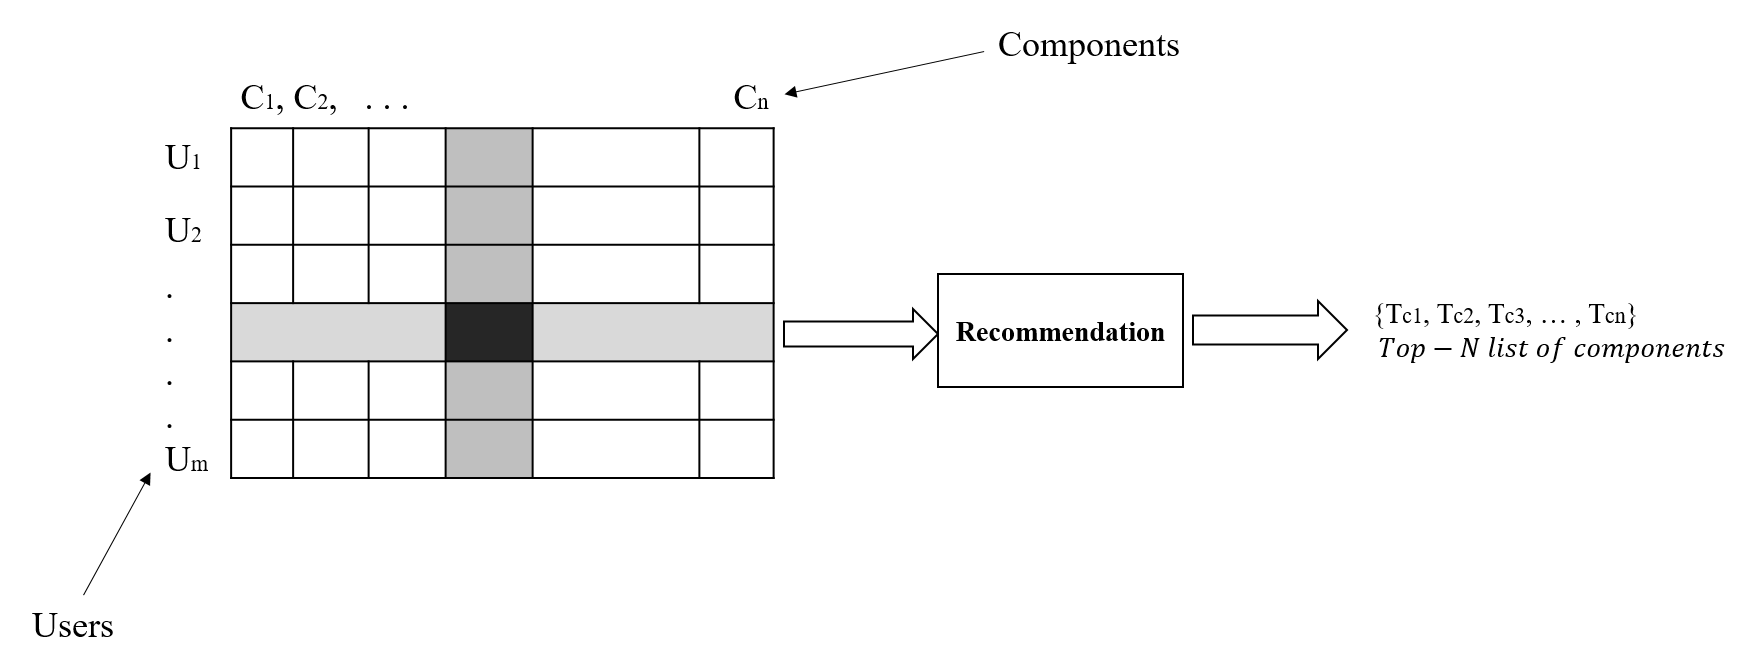
\includegraphics[width=0.75\linewidth]{./collaborative-filtring.png}
	\vspace*{-3pt}
	\caption{Collaborative Filtering Process for Identifying Most Important components}
	\label{fig:collabrotaivefiltering}
\end{figure*} 
The goal of our hybrid recommender method is to suggest the highest risky 
components with most frequency among all other components in the applications. 
To do this we used  two collected datasets: 
user sessions $U=\{u_1, u_2, ... , u_m\}$ and 
list of our components $C =\{c_1, c_2, ... , c_n\}$. Each user $u_i$ 
has a list of components $c_{ui}$ which the user
has performed at least one task on that particular $c$. \\
Generally in recommender systems prediction is based on the numerical value of 
rating from an active user, while in our case we do not have a access to such rating 
module instead we assume the value of frequency access for a specific component by 
an individual active user as a rating score. \\
There are two main techniques for collaborative filtering algorithms:
Memory based (user-based) and Model based (item-based) algorithms. 
In memory based collaboration filtering we seek to find the 
most similar users to the current active user while in the model based algorithm 
first we design a model of users rating and then we will evaluate 
the expected rating of an item based on the previous rating of the other similar items.\\  
%Many machine learning algorithm can be applied to identify the probability of rating for 
%each item, among x, x, and x we applied x because of x. \\
The item based approach looks into the set of items the target user has rated and computes 
how similar they are to the target item i and then selects $k$ most similar items $\{i_1, i_2, ..., i_k\}$.
At the same time their corresponding similarities $\{s_{i1}, s_{i2}, ..., s_{ik}\}$ are also computed. 
Once the most similar items are found, the prediction is then computed by 
taking a weighted average of the target users's rating on these similar items. 
In order to determine similarity between two components $i$ and $j$ we used
Pearson-r correlation. 
If $U$ is the set of users who rated $i$ and $j$ then we compute the correlation similarity by

%\[
%{Sim (i,j) = \frac {\sum_{u\in {U}}(C_{u,i} - \bar{C_i})(C_{u,j} - \bar{C_j)}}{ \sqrt{\sum_{u\in {U}}({C_{u,i} - C_i})^{2}}{ \sqrt{\sum_{u\in {U}}({C_{u,j} - \bar{C_j}})^{2}}}}}	
%\]

\[
{Sim (i,j) = \frac {\sum_{u\in {U}}(C_{u,i} - \bar{C_i})(C_{u,j} - \bar{C_j)}}
	{ \sqrt{\sum_{u\in {U}}({C_{u,i} - \bar{C_i}})^{2}}
	{ \sqrt{\sum_{u\in {U}}({C_{u,j} - \bar{C_j}})^{2}}}}}	
\]


where $C_{u,i}$ is the value of frequency access of user u on the component $i$, 
$\bar{C_i}$ is the average value of frequency for the $i-th$ component . 


\[
{P_{u,i} = \frac {\sum_{{all\: simillar\: components , N}}(S_{i,N} * R_{u,N})}
	{\sum_{{all\: simillar\: components, N}}({S_{i,N}})}}
\]

In order to estimate the rate of ignored components we will conduct 
ratio prediction computation by using weighted sum method. 
This method provides the ratio prediction of a specific component i 
for user u based on similar components to i. 
this method will return how a user rates the similar items. 


\subsubsection{Workflow of Recommender system}

In figure ~\ref{fig:workflow} we depict the workflow of our proposed technique. 
The workflow steps are as follows:\\
1) Users sessions collection: This module collect the telemetry data 
from users interaction. The obtained information are:user name, 
date, action name and page name. \\
2) Change history collection: This module obtains change history 
for each component. In section xx we describe the metrics and process 
of change history collection. \\
3) Determine the most frequent components: This module calculate the most 
access component based on users interaction. To compute the frequency score we 
applied to different techniques which have been explained in section xx.\\
4) Components similarity computation: In order to measure similarity between two 
component we used Pearson-r correlation formula which we described above.\\
5) Ranking components:Normally in CF recommender system there is a prediction step 
which calculate the probability of most similar item for an active user since, 
the focus of our study is identifying the most risky component we eliminate that step. 
Using the below formula we can calculate the ranking score for each component: 
\[
{ R_{Ci} = F_{Ci} * W_{Ci}}	
\]

where $F_{Ci}$ is the frequency score of component $i$ and $W_{Ci}$ is the weight of $C_i$.  

6) Test case recommendation: The final step of our recommender system is reordering
our test cases based on their coverage of $Top-N$ components. 

\begin{figure}[t]
	\centering
	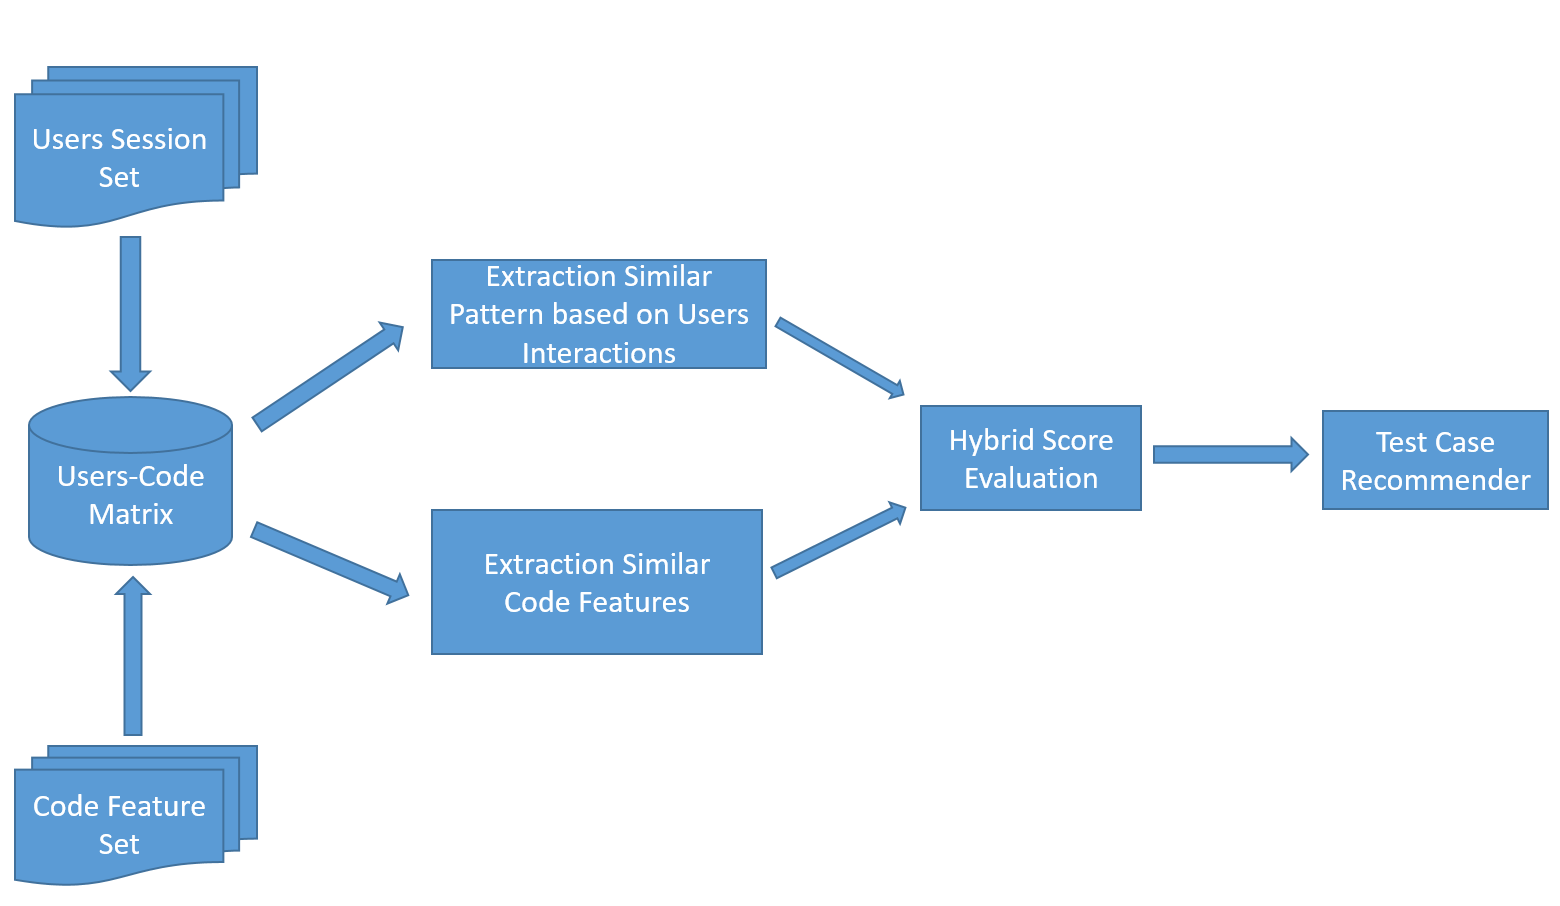
\includegraphics[width=0.90\linewidth]{./Overview.png}
	\vspace*{3pt}
	\caption{The workflow of the proposed risk evaluation method}
	\label{fig:workflow}
\end{figure}


\subsection{Control Techniques}





\vspace*{4pt}
\section{Empirical Study}
\label{sec:study}

%As stated in Section \ref{sec:introduction}, the goal of
%this study is to assess our regression testing approach in terms 
%of the detecting high risk component.
%In particular, we address the following research questions:

%\begin{itemize}
%\item[RQ1:] Is there any common subset of metrics which is applicable to 
%predict regression defects in different projects?
%\item[RQ2:] Are final scores effective at identifying high risky classes?
%\item[RQ3:] Can our recommender system be useful for 
%improving performance regression testing techniques?
%\end{itemize}

\noindent


%\subsection{Hypothesis}
%\begin{itemize}
%	\item[H1] Increase in complexity metrics of a component C correlates with
%	the regression of C.
%	\item[H2] Having change history of a component C 
%	is a evidence for risk of future regression of C.
%	\item[H3] There is a relation between number of 
%	interactions of a class C to the regression of C.
%\end{itemize}


\subsection{Objects of Analysis}
\label{sec:objects}

To investigate our research questions, we performed
an empirical study.
The following subsections present our objects of analysis, 
study setup, threats to validity, and data analysis.

%In this study, we used five open source web applications
%written in PHP as objects of analysis; the applications
%were obtained from SourceForge.
%
\begin{table}
	\caption{Subject Applications properties}
%	\vspace*{-10pt}
	\begin{center}
		\begin{tabular}{|l||c||c||c||c|}
			\hline
			Metrics  & DASCP & MixERP & nopCommerce & Coevery \\\hline
			Classes   & 107  & 5,760 & 1,919& 2,258 \\\hline
			Files  & 201  & 5,473 & 1,473 & 1,875 \\\hline
			Functions & 940  & 57,594 & 21,057 & 13,041 \\\hline
			LOC &   35,122  & 837,674  & 226,354 &120,897 \\\hline
			Sessions  & 748 &  xx&xx &xx\\\hline
			Faults  & 35 &  xx& xx&xx\\\hline
			Version  & 3 &  5 & 23 & 3 \\\hline
			Test Cases & 95& 21 & 543 & 1,120\\\hline
			Installations & 3 & 1  & 2 & 1 \\\hline
		\end{tabular}
		\end {center}
		\label{tab:AUTs}
%		\vspace*{-5pt}
	\end{table}


\subsection{Variables and Measures}
\label{sec:measures}

\subsubsection{Independent and Dependant Variables}
\label{sec:independent}


Independent variables in our study are the user-session-based test suites,
the seeded faults and the test case prioritization techniques.
Dependent variables are rate of fault detection, 
average percent of faults detected (APFD) [xx], and test execution time.

%\subsubsection{Dependent Variable and Measures}
%\label{sec:dependent}
%
%Our dependent variable is the number of test paths generated
%by the techniques.


\section{Experiment Setup}
\label{sec:setup}


In this section, we describe applied techniques to examine different types of
test prioritization techniques. Our Study contains three main categories:\\
\textbf{User Session based Prioritization}
In this experiment we reorder our test cases that cover 
most frequently used web pages. Assume $(T, S, M, f, A)$, where $T$ is the set of 
test cases, $S$ is the collection of user session, $M$ is applied method, $f$ is the frequency score 
based on $M$ and $A$ is Average percentage of fault detection, 
the desired output is to reorder $T$ based on $f$ where $A$ obtains higher value 
compare to its default value which is a random.\\
\textbf{Change History based Prioriitization}
% reason why change hsitory is important based on previous study
We used the change history of our AUTs to determine most risky 
components then we reorder the test cases based on 
the ascending value of risk for each component. \\
\textbf{Hybrid Recommendation Method} 
In our third study we proposed a hybrid method which use
the users interaction data and change history. We draw 
similarity matrix  based on those information to find the 
most risky and frequently used web page in our web application. 
Afterward, we change the order of our test cases based on output of our recommender system. \\

\subsection{User Session based Prioritization}
Our first test prioritization is based on the information we 
collected from monitoring our volunteer users. 
We asked hundred volunteer users whom are computer science students from 
University of North Texas and we asked the to perfome variety of tasks in our applications. 
Among all collected information,  we applied two main techniques to 
figure out most frequent parts of our applications. Below we describe these two techniques:

\subsubsection{Most Frequent Web Pages}
this approach determines the most frequent web pages that have been used by users. 
We assume that the most frequent web pages are playing more important role in the system, 
eventually, they should have a higher priority to be test first. Another reason
 of why frequency of web pages is the key for testing is most frequent web pages usually 
 contains more functionality and connections with other pages, so any bug in 
 those pages can effect higher portion of the entire system. 
 Here we define base session as a session that provided by our users 
 and covers the most interactions in the application.
 we picked 20 percent of our total sessions as a base session. 
 For example, in online shopping, our base session is a sequence of actions from user login to check out, including all necessary actions and some random unnecessary such as browsing other items, checking inbox during shopping process etc. 
 \begin{figure}[t]
 	\centering
 	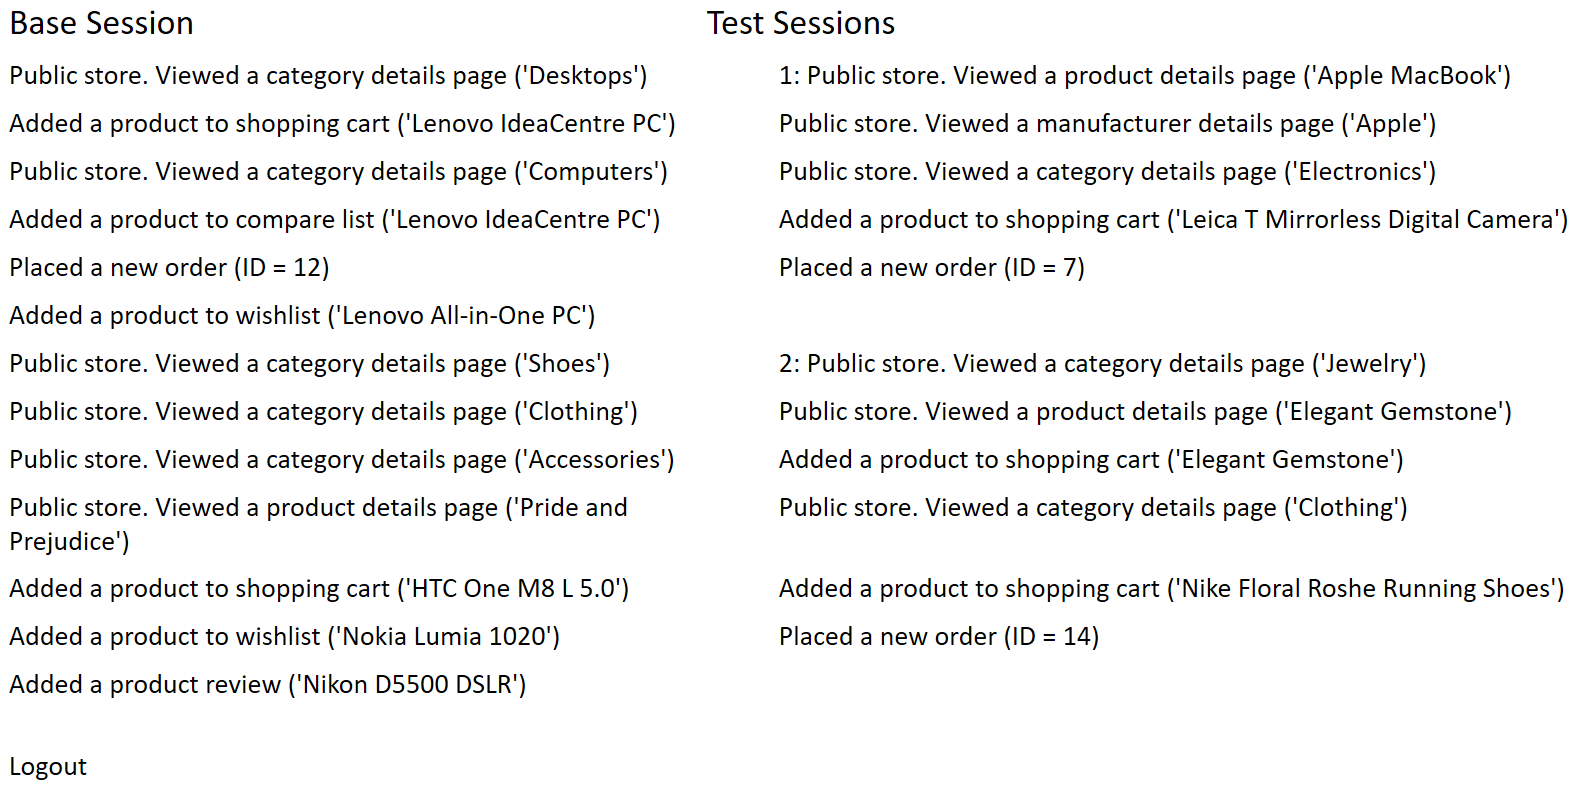
\includegraphics[width=0.90\linewidth]{./SessionSample.png}
 	\vspace*{3pt}
 	\caption{Sample of Base Session and Test Sessions}
 	\label{fig:sessions}
 \end{figure}

After collecting all sessions, we condoct an analysis of web pages frequency 
by comparing obseverd web pages in each session with base session. 

\[
{F_{w,i} = \frac {\sum_{{page\: score\: for \: each\: session}}(S_{i})}
	{\sum_{{number \: of \: base \: sessions}}({BS_{i}})}}	
\]

Using figure ~\ref{fig:sessions} as an example, page x from base session 
have been observed in both test session 1 and 2. If we assume we have 10 test session and 3 base sessions
and this particular page have been observed in 7 of the 10 pages then, frequency of page x is equal to 
$(0.7 / 3) = 0.23$

\subsubsection{Most Frequent Actions}
Most frequent actions typically are the main functions in the system and in a 
normal case they contain high dependency to the other classes and functions. 
If one main function fails it can be cause of a significant failure or degrade of the system. 
Another factor of importance of most frequent functions is to prevent of domino effect in the system. 


\subsection{Change History based Prioriitization}
Among hundreds attribute of code and change history to evaluate the code quality and 
error proness we choose change history to identify most risky web pages. In previous 
study [ref Raimund] shows the role of change history in bug detection and its superiority 
in terms of bug detection. In this study we collect the change history of our three applications. 
We chose xx metrics based on their correlation to the previous observed bugs.
Also most of these metrics have been used in [,,,,] as a feature for bug detection. 
Table xx shows the applied change metrics in this study. 

	\begin{table}
	\caption{Change metrics used to evaluate risk in this study}
	\begin{tabular*}{.4\textwidth}{c @{\extracolsep{\fill}} |ll}
	\hline
	Metrics name & Description \\\hline
	Revision & Number of revision of a component  \\\hline
	LOC Added&   Added lines of code \\\hline
	Max LOC Added  & Maximum added lines of code \\\hline
	AVE LOC Added  & Average added lines of code \\\hline
	LOC Deleted  & Deleted lines of code  \\\hline
	Max LOC Deleted & Maximum deleted line\\\hline
	AVE LOC Deleted & Average deleted lines of code \\\hline
	Code Churn & sum of change in all revisions \\\hline
	Age & Age of the component in days from last release \\\hline
	Time & Time of the change in dd-mm-yyyy format \\\hline		
	\end{tabular*}
		\label{tab:historyMetrics2}
	\end{table}
		

After the change history data collection, we applied ANOVA analysis on our dataset to attain a linear model.
Our aim is to find the correlation coefficient for each metric to measure statistical relationships between 
a variable and real defects. The value of this measure fluctuate between 1 and -1. Here 1 indicates strong 
positive relationship which means increase in variable values, increases the output value, 0 shows no correlation 
and negative value means revers correlation. 
Other than that, we calculated root mean squared error and mean absolute error. 
The lower error value shows that the model has higher prediction accuracy. 
Our label in the dataset is the bug reports. Note that our web pages are 
dynamic and they contain a class code behind which is the main concern in our study not HTML bugs. 

In order to evaluate our linear model, we applied 10-fold cross validation. 
In next step we applied our obtained model to evaluate the riskiness of each component. 

\subsection{Hybrid Recommendation Method}



\section{Study}
\subsection{Object of Analysis}
\subsection{Variables and Measures}
\subsection{Data Collection and Experimental Setup}

\section{Threats to Validity}
\label{sec:validity}


%In this section, we describe the internal and external
%threats to the validity of our study. We also describe 
%the approaches we used to limit the effects of these threats.
%
%{\em Internal Validity:}
%The outcome of our study could be affected by the choice of 
%program analysis. We applied static analysis on a dynamic programming 
%language, PHP. To do so, we had to change many statements in the 
%program during the file preparation phase, removing and fixing 
%many dynamic environment variables. However, we carefully examined 
%our process to minimize the adversary effect that might be introduced
%into the converted files.  
%
%{\em External Validity.}
%We used open source web applications for our study, so these programs 
%are not representative of the applications used in practice, and thus
%we cannot generalize our results. However, we tried to reduce this 
%threat by using five non-trivial sized web applications with multiple 
%versions that have been utilized by many users. 




